\documentclass[a4paper, 11pt, onecolumn]{article}
\usepackage{fullpage} % changes the margin
\usepackage{amsmath}
\usepackage{graphicx}
\usepackage{layouts} % allows printing the value of \textwidth for matplotlib
\usepackage{multicol}
\usepackage{physics}

\usepackage{wrapfig}
\usepackage{floatflt}



\begin{document}
\title{Falikov-Kimball Project Notes}
\author{Thomas Hodson}
\maketitle

\section{Objectives}
We would like to study the generic physics of finite temperature phase transitions (FTPTs). It's preferable to do this in 1D as it admits simpler numerical and analytic analysis while still describing experimental relevant systems. However, from Peierls' argument \cite{peierls_isings_1936}, one dimensional models with short ranged interactions cannot have an FTPT because entropic effects always outweigh energetic effects. We therefore study 1D models with long range interactions, which can support FTPTs \cite{dyson_existence_1969,thouless_long-range_1969,anderson_exact_1969}. The first such model we are looking at is the 1D Falikov-Kimball (FK) Model, modified to include long range interactions. I've written code to simulate this model with Markov Chain Monte Carlo (MCMC). 

\section{Fermi-Hubbard Model}
Mostly from cond-mat.de/events/correl16/manuscripts/scalettar.pdf

With annihilation and creation operators for a spin 1/2 fermion:
\begin{multicols}{3}
\noindent
  \begin{equation*}
    \{c_{i\sigma}, c^\dag_{j,\rho}\} = \delta_{ij}\delta_{\sigma \rho}
  \end{equation*}
  \begin{equation*}
    \{c_{i\sigma}, c_{j,\rho}\} = 0
  \end{equation*}
    \begin{equation*}
    \{c^\dag_{i\sigma}, c^\dag_{j,\rho}\} = 0
  \end{equation*}
\end{multicols}

\begin{wrapfigure}{l}{0.3\textwidth}
  \begin{center}
    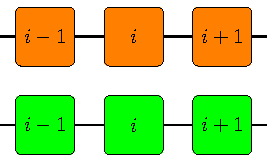
\includegraphics[width=0.25\textwidth]{FH_diagram}
  \end{center}
  %\caption{The Fermi-Hubbard model with the two spin states represented by }
\end{wrapfigure}

The Fermi-Hubbard (FH) model (Original paper \cite{hubbard_j._electron_1963}, Review \cite{manousakis_spin-textonehalf_1991}, Phase Diagram: \cite{esslinger_fermi-hubbard_2010}, Cold atom simulation \cite{mazurenko_cold-atom_2017}) describes spin $\frac{1}{2}$ fermions on a lattice with nearest neighbour interactions characterised by an energy scale $t$, on-site interactions by $U$ and chemical potential $\mu$. It's not actually necessary for these to be spin 1/2 particles, only that there are two species which are distinguishable in some way.

$$ H = -t \sum_{<ij>,\sigma} c^\dag_{i\sigma}c_{j\sigma} + U \sum_{i} n_{i \uparrow} n_{i\downarrow} - \mu \sum_i \left( n_{i \uparrow} + n_{i \downarrow} \right)$$

with the number operator defined as usual: $n_{i \sigma} = c^\dag_{i\sigma}  c_{i\sigma}$

\subsection{Particle-Hole Symmetry}
On bipartite lattices (square, hexagonal, linear chain...), latices points can always be partitioned into two sublattices such that every point site is neighboured by sites from the opposite sublattice. The Hubbard model on a bipartite lattice is symmetric under a Particle Hole (PH) transformation which exchanges creation and annihilation operators while also adding an alternating signs between the two sublattices.

$$ d^\dag_{i\sigma} = (-1)^i c_{i\sigma}$$
The number operator $n_{i\sigma} = 0,1$ now counts holes rather than particles:
$$ d^\dag_{i\sigma} d_{i \sigma} = c_{i\sigma} c^\dag_{i\sigma} = 1 - c^\dag_{i\sigma} c_{i\sigma}$$
With the last equality following from the commutation relations. In the case of nearest neighbour interactions on a bipartite lattice this transformation also leaves the hopping term unchanged:
$$ d^\dag_{i\sigma} d_{j \sigma} = (-1)^{i+j} c_{i\sigma} c^\dag_{j\sigma} = c^\dag_{i\sigma} c_{j\sigma}$$
By definition, when $i$ and $j$ label sites on separate sublattices, $(-1)^{i-j} = -1$ and this is absorbed into rearranging the operators via their anti-commutator.

Rewriting the original Hamiltonian makes the symmetry clear:

$$ H = -t \sum_{<ij>,\sigma} c^\dag_{i\sigma}c_{j\sigma} + U \sum_{i} (n_{i \uparrow} - 1/2)( n_{i\downarrow} - 1/2) - (\mu - U/2) \sum_i \left( n_{i \uparrow} + n_{i \downarrow} \right) - N U/4$$
Shifting the chemical potential $\mu^* = \mu - \frac{U}{2}$ and neglecting the additive constant:

$$ H(t, U, \mu^*) = -t \sum_{<ij>,\sigma} c^\dag_{i\sigma}c_{j\sigma} + U \sum_{i} (n_{i \uparrow} - 1/2)( n_{i\downarrow} - 1/2) - \mu^* \sum_i \left( n_{i \uparrow} + n_{i \downarrow} \right) $$
Defining the particle density $\rho$ as the number of fermions per site:
\begin{multicols}{2}
\noindent
  \begin{equation*}
    \rho = \frac{1}{N} \sum_i \left( n_{i \uparrow} + n_{i \downarrow} \right)
  \end{equation*}
  \begin{equation*}
    0 < \rho < 2
  \end{equation*}
\end{multicols}

The PH symmetry maps the Hamiltonian to itself with the sign of the chemical potential reversed (and an additive constant) and the density is inverted about half filling:
$$ \text{PH} : H(t, U, \mu*) \rightarrow H(t, U, -\mu*) $$
$$ \rho \rightarrow 2 - \rho $$

So for $\mu^* = 0$ the Hamiltonian is symmetric under PH and so must all the observables, hence half filling $\rho = 1$ occurs here. I'll drop the star on $\mu^*$ at this point.

\subsection{Momentum Space}
The particle hole symmetry in momentum space:
$$ c^\dag_{k\sigma} \equiv \frac{1}{\sqrt{N}} \sum_n e^{ikna} c^\dag_{n\sigma}$$

\begin{align*} 
PH: c^\dag_{k\sigma} &\rightarrow  \frac{1}{\sqrt{N}} \sum_n e^{ikna} (-1)^n c_{n\sigma} = \frac{1}{\sqrt{N}} \sum_n e^{i(k + \pi/a)na} c_{n\sigma} \\
&= c_{k+\pi/a,\sigma} \\
PH: c^\dag_{k\sigma} &\rightarrow c_{k+\pi,\sigma} \\
\end{align*}

\begin{figure}
  \centering
    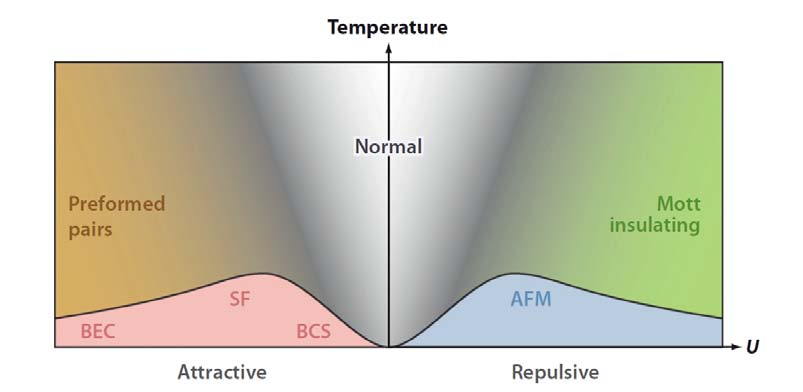
\includegraphics[width=0.8\textwidth]{FH_phase_diagram}
  \caption{Phases of the Fermi Hubbard mode from \cite{\cite{esslinger_fermi-hubbard_2010}}}
  \label{fig:FH_phase_diagram}
\end{figure}

\section{Falikov-Kimball model}
The FK model  \cite{falicov_simple_1969} can be obtained by giving the Fermi-Hubbard model spin dependent hopping terms. 
$$ H(t, U, \mu) = -\sum_{<ij>,\sigma} t_{\sigma} c^\dag_{i\sigma}c_{j\sigma} + U \sum_{i} (n_{i \uparrow} - 1/2)( n_{i\downarrow} - 1/2) - \mu \sum_i \left( n_{i \uparrow} + n_{i \downarrow} \right) $$


\begin{wrapfigure}{R}{0.3\textwidth}
  \begin{center}
    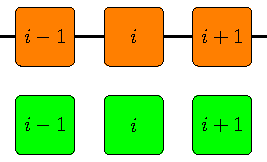
\includegraphics[width=0.25\textwidth]{FK_diagram}
  \end{center}
  %\caption{The Fermi-Hubbard model with the two spin states represented by }
\end{wrapfigure}
Setting the hopping to zero for one of the spin directions/species causes it to become immobile and effectively classical. The local number operator \(n_{i\downarrow} \equiv n^f_i\) commutes with the Hamiltonian and therefore any real space configuration is conserved over time.

$$ H(t, U, \mu) = -\sum_{<ij>} c^\dag_{i\uparrow}c_{j\uparrow} + U \sum_{i} (n_{i \uparrow} - 1/2)( n_{i\downarrow} - 1/2) - \mu \sum_i \left( n_{i \uparrow} + n_{i \downarrow} \right) $$

Conventionally one one would present this as a model with two separate species of particle: immobile, classical f-electrons and itinerant, quantum c-electrons.

$$ H = - t\sum_{<ij>} c^\dagger_ i c_j + U \sum_i (c^\dagger_ i c_i - 1/2)(n^f_i - 1/2) - \mu \sum_i (c^\dagger_ i c_i  + n^f_i) $$

The FK model inherits the same particle-hole symmetry as the Fermi-Hubbard model, so with this definition of $H$ and $\mu$ we can say by symmetry that $\mu = 0$ gives falf filling for all $T, U$.

\subsection{Periodic Anderson Model}
\begin{wrapfigure}{l}{0.3\textwidth}
  \begin{center}
    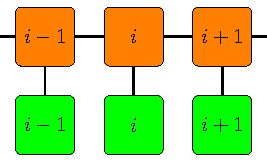
\includegraphics[width=0.25\textwidth]{PAM_diagram}
  \end{center}
\end{wrapfigure}

As a quick aside, the Periodic Anderson Model (PAM) is similar to the FK model, the two differences being that there are two bands (d and c) and the fermions are spin 1/2, giving four operators per site rather than two in the spinless FK model. Secondly hopping is allowed between the bands. One of the bands remains dispersionless/localised like the f electrons in the FK model.

\begin{align*} H = &- t\sum_{<ij>\sigma} c^\dagger_{i\sigma} c_{j\sigma} + c^\dagger_{j\sigma} c_{i\sigma} + K\sum_{<ij>\sigma} c^\dagger_{i\sigma} d_{j\sigma} + d^\dagger_{j\sigma} c_{i\sigma} \\
&+ U \sum_{i\sigma} (c^\dagger_ {i\sigma} c_{i\sigma} - 1/2)(d^\dagger_ {i\sigma} d_{i\sigma} - 1/2) - \mu \sum_{i\sigma} (c^\dagger_ i c_i  + d^\dagger_ i d_i)
\end{align*}


\section{Phases of the 2D Falikov Kimball Model}

\begin{wrapfigure}{r}{0.5\textwidth}
  \centering
    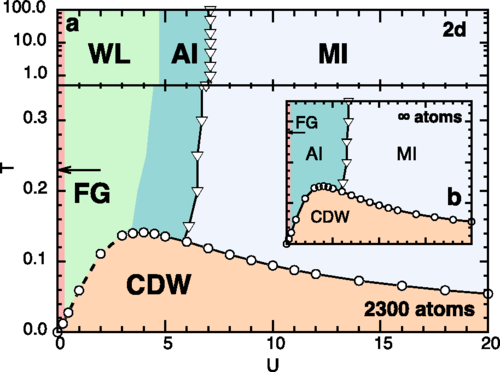
\includegraphics[width=0.4\textwidth]{phase_diagram}
\end{wrapfigure}

The phase diagram of the 2D FK model at half filling calculated from Monte Carlo simulations \cite{antipov_interaction-tuned_2016} is shown on the right. The phases are related to those of the FH model, the charge density wave state (CDW) maps directly onto the antiferromagnetic order in the FH model. At large U a similar Mott insulating phase appears. In the Anderson insulator phase (AI) the c electron wavefunctions are localised by the disordered f electrons. In the weakly localised phase the localisation length approaches the system size, so this phase is absent in the thermodynamic limit (inset). 



\subsection{Large U limit: The Mott Insulating phase}

In the limit $U \rightarrow \infty$ such that the hopping terms can be ignored, the FK and FH models are the same. The problem essentially becomes a single site problem as the eigenvectors become products of the single site eigenvectors $\ket{n, 0}, \ket{n, \uparrow}, \ket{n, \downarrow}, \ket{n, \uparrow \downarrow}$

\begin{align*} Z &= \Tr e^{-\beta \hat{H}} = \sum_{i} \ev{e^{-\beta \hat{H}}}{\psi_i} \\ 
&= e^{-\beta (U / 4)} + 2e^{-\beta (-U/4 - \mu)} + e^{-\beta(U/4 - 2\mu)}
\end{align*}

$$\rho = \frac{1}{Z}\Tr\left[ (n_{\downarrow} + n_{\uparrow}) e^{-\beta \hat{H}} \right] = \frac{1}{Z} (2e^{-\beta (-U/4 - \mu)} + 2e^{-\beta(U/4 - 2\mu)})$$


\begin{figure}
  \centering
    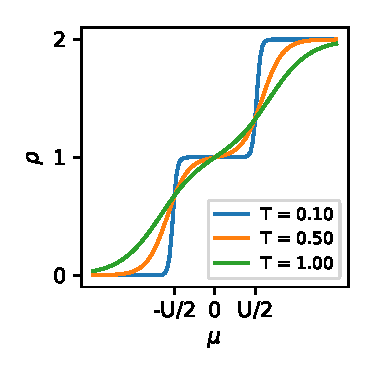
\includegraphics[width=.5\textwidth]{single_site_limit.pdf}
  \caption{Single site limit. U = 4. Around $\mu = 0$ the compressibility $\frac{\partial \rho}{\partial \mu} = 0$, a Mott insulator.}
  \label{fig:single_site_limit}
\end{figure}

The system has a Mott plateau around $\mu = 0$ which creates an interaction mediated insulating phase


\subsection{Fermi Gas}
When U = 0, the problem just boils down to a non-interacting Fermi gas.

\subsection{Anderson insulator}

\subsection{Charge density waves}
The the f-electrons form a charge density wave (CDW) \cite{antipov_interaction-tuned_2016,herrmann_spreading_2018}.

\section{Adding Long-ranged interactions to the 1D Falikov Kimball Model}

In one dimension Peierls' argument \cite{peierls_isings_1936, kennedy_itinerant_1986} makes it clear that short range interactions can never overcome entropic effects to stabilise an ordered phase at finite temperature so the FK model has no CDW phase in 1D.

\subsection{Peierls' argument and domain walls}
Peierls' argument considers an ordered state in a 1D short-ranged system. In short ranged systems, the energy cost of a domain wall $E_0$ doesn't grow with system size, while the entropy associated with adding a domain wall into any position in a system with N sites is $\Delta S = k_B \ln (N - 1)$. 
In the thermodynamic limit the entropic term will at some point outweigh the energy penalty, i.e $\Delta F = E_0 - T\Delta S < 0$ so domain walls will proliferate and destroy any long range order in 1D.

The argument fails for long ranged interactions, consider a ferromagnetic Ising model:
\begin{multicols}{2}
\noindent
  \begin{equation*}
    H = - \sum_{<ij>} J(|i-j|) s_i s_j
  \end{equation*}
  \begin{equation*}
    J(x) = x^{-\alpha}
  \end{equation*}
\end{multicols}

The energy cost of introducing a single domain wall onto a ferromagnetically ordered state in 1D is 
$$E \propto \sum_{n=1}^{\infty} n J(n)$$
because each interaction between spins separated across the domain by a bond length $n$ can be drawn between $n$ equivalent pairs of sites. Ruelle (1968) \cite{ruelle_statistical_1968} proved rigorously for a very general class of 1D systems, that if $E$ or its many-body generalisation converges in the thermodynamic limit then the free energy is analytic. This rules out a finite order phase transition, though not one of the Kosterlitz-Thouless type. Dyson \cite{dyson_existence_1969} also proves this though with a slightly different condition on $J(n)$.

With a power law interaction, there are three cases to consider:

\newline
\begin{center}
    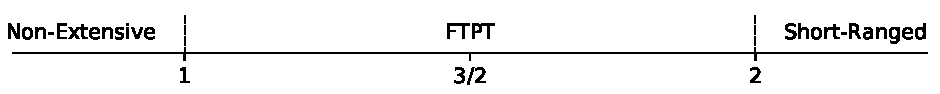
\includegraphics[width=\textwidth]{alpha_diagram}
\end{center}

\newline

\begin{itemize}
    \item \( \alpha = 0\) For infinite range interactions the Ising model is exactly solve-able.
    \item \( \alpha \le 1\) For slowly decaying interactions $\sum_n J(n)$ does not converge so the Hamiltonian is non-extensive.
    \item \( 1 < \alpha < 2 \)  The case we're looking at here will be the intermediate one, which has a phase transition to an ordered state at a finite temperature.
    \item \( \alpha = 2 \) the energy of domain walls diverges logarithmically, turns out to be the Kostelitz-Thouless transition. (find a good citation for this)
    \item \( 2 < \alpha \) For quickly decaying interactions, domain walls have a finite energy penalty, hence Peirels' argument holds and there is no phase transition.


\end{itemize}

\subsection{Adding long range interactions to the FK model}

The FK model can be viewed as a model of itinerant electrons (the c-electrons) coupled to an Ising model (the f-electrons). From this point of view the CDW state is an antiferromagnetic spin state. To produce the CDW state in the 1D model we add 

  \begin{equation*}
    H_{\textrm{int}} = \sum_{ij} J\left(|i-j|\right) \left( n^f_i - \frac{1}{2} \right) \left( n^f_j - \frac{1}{2} \right)
  \end{equation*}
  \begin{equation*}
  J(n) = J^* \frac{(-1)^n}{ n^{\alpha} }
  \end{equation*}
  \begin{equation*}
    1 < \alpha < 2
  \end{equation*}

This is:
\begin{itemize}
    \item Long ranged, bypassing Peirels' argument.
    \item Staggered by $(-1)^n$ so that antiferromagnetic/CDW order is favoured.
    \item Particle hole symmetric, as the $\mathbb{Z}_2$ symmetry of the Ising model maps to the particle-hole symmetry of the FK model.
\end{itemize}

\section{Analytic treatments}
\subsection{Low temperature limit}

In the limit of low temperature the f-electrons form a completely static CDW which can be treated as a periodic potential for the c-electrons, leading to the usual opening of a band gap in the c-electron spectrum, shown in Figure \ref{fig:dos}(b).

\subsection{Uncorrelated Noise}
For finite temperatures, the CDW is not static but starts to contain correlated noise, so the energy spectrum and density of states are modified from that shown in Figure \ref{fig:dos}. As a sanity check \ref{fig:dos}(c) shows the effect of adding uncorrelated perturbations about a CDW state. 

\subsection{Ising Model mean field}

\begin{figure}
  \centering
    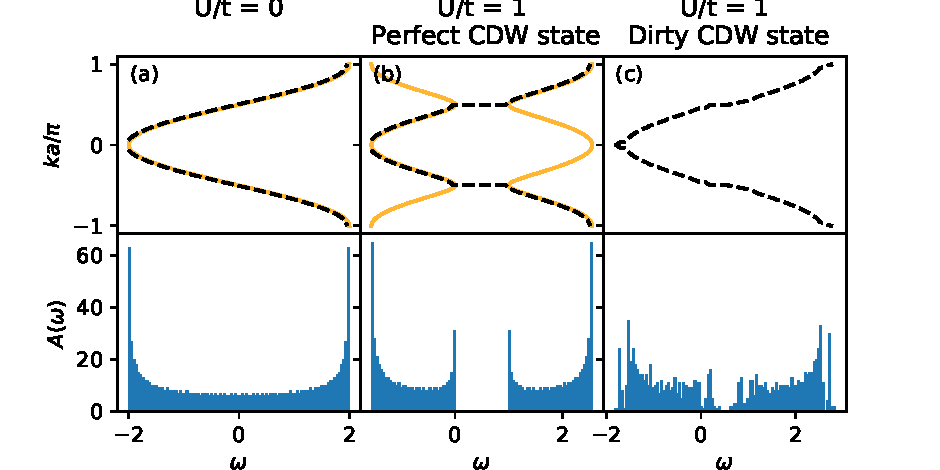
\includegraphics[width=\textwidth]{DoS.pdf}
  \caption{The Energy Spectrum $k(\omega)$ and Spectral function $A(\omega)$ of the c-electron Hamiltonian. Obtained by diagonalising a system with $N = 128$ with 100 separate disorder realisations: The energy spectrum is calculated numerically (black) and the analytic result where available is shown in orange. (a) The free fermion case. (b) When U = t and the f-electrons are in a static CDW state, the c-electrons see a periodic potential and a band gap opens. (c) If each of the CDW sites is inverted with 10\% probability, the energy spectrum is smoothed out and states appear within the bandgap.}
  \label{fig:dos}
\end{figure}

\section{Monte Carlo simulations}
Because the f electrons are classical, it is possible to efficiently sample from a thermal distribution over f-electron states:


$$ Z = \Tr e^{-\beta H} $$

At half filling, define the classical part of the Hamiltonian as the part which is composed solely of number operators of the f-electrons.

$$ H_{\text{classical}} = -U/2 \sum_i n^f_i + H_{\text{int}}$$

$$ H_{\text{non-classical}} = - t \sum_{<ij>} c^\dagger_i c_j + U \sum_{i} c^\dagger_i c_i (n^f_i - 1/2) $$

For a given configuration of the f electrons, call it  \(\{ n^f_i \}\)  the energy from the classical Hamiltonian is easy to calculate because all the operators have definite values. For the rest of the Hamiltonian we still have to diagonalise and carry out a proper trace.

$$ Z = \sum_{\{ n^f_i \}} e^ {\beta H_{\text{c}}} \Tr e^{-\beta H_{\text{nc}}} $$

Markov chain Monetcarlo is used to sample from the distribution $\propto Z$ in the space of f-electron configurations. Will flesh this out more.


\begin{figure}
  \centering
    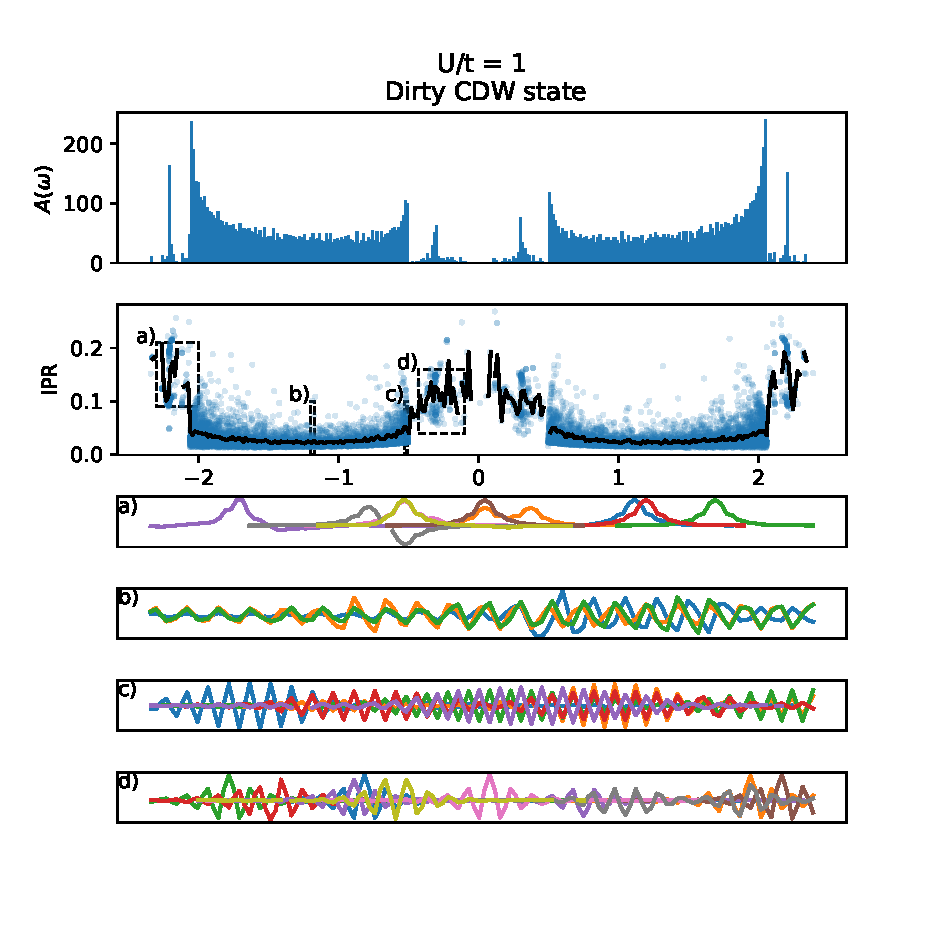
\includegraphics[width=\textwidth]{States}
  \caption{The Spectral function $A(\omega)$ and Inverse Participation Ratio (IPR) of the c-electrons. Obtained by diagonalising a system with $N = 1000$ about a dirty CDW state with 5\% of the sites flipped uniformly. The wavefunctions that appear within the gap (d) and outside the usual band edges (a) are localised, while those within the conventional bands seem less localised. }
  \label{fig:states}
\end{figure}

\begin{figure}
  \centering
    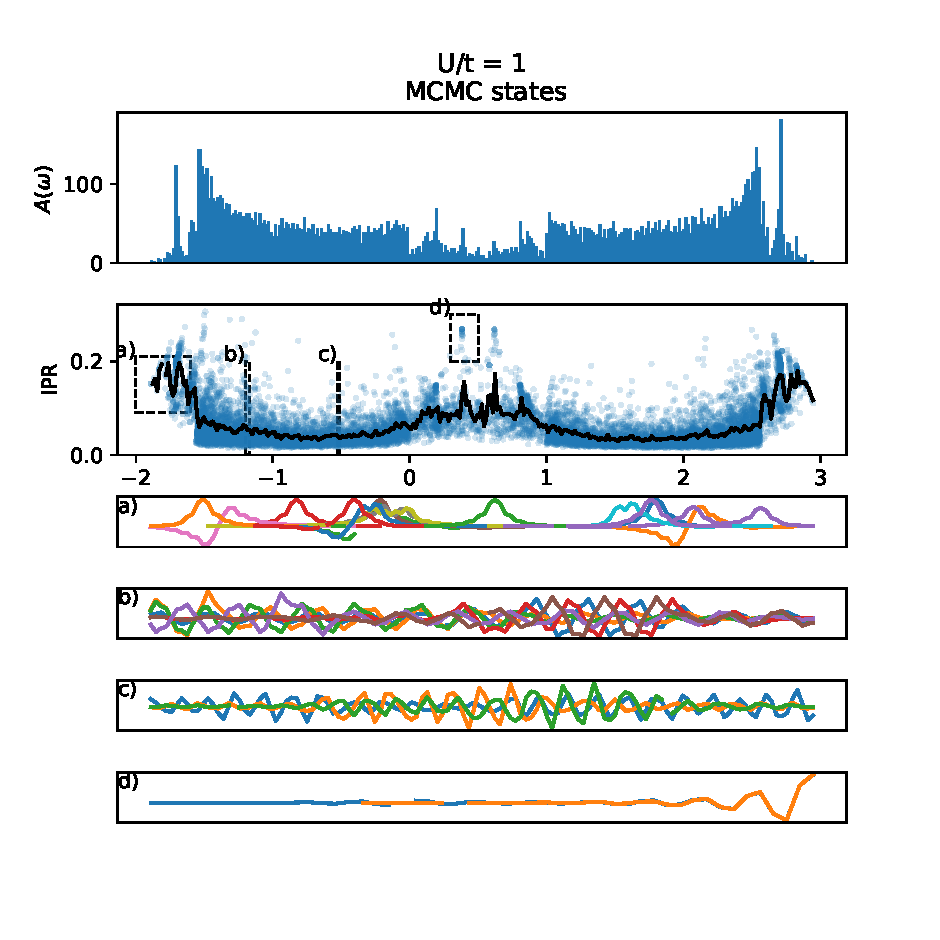
\includegraphics[width=\textwidth]{mcmc_States}
  \caption{The Spectral function $A(\omega)$ and Inverse Participation Ratio (IPR) of the c-electrons. The system size $N = 128, \alpha = 1.5, J^* = 1, \beta = 0.7$ with 100 samples plotted from a Montecarlo run of 1000 samples. This figure differs from Fig \ref{fig:states} in that the results are thermal averages obtained through MCMC from the full partition function. plots a-d show the sample wavefunctions from different regions of the plot.}
  \label{fig:mcmc_states}
\end{figure}

\begin{figure}
  \centering
    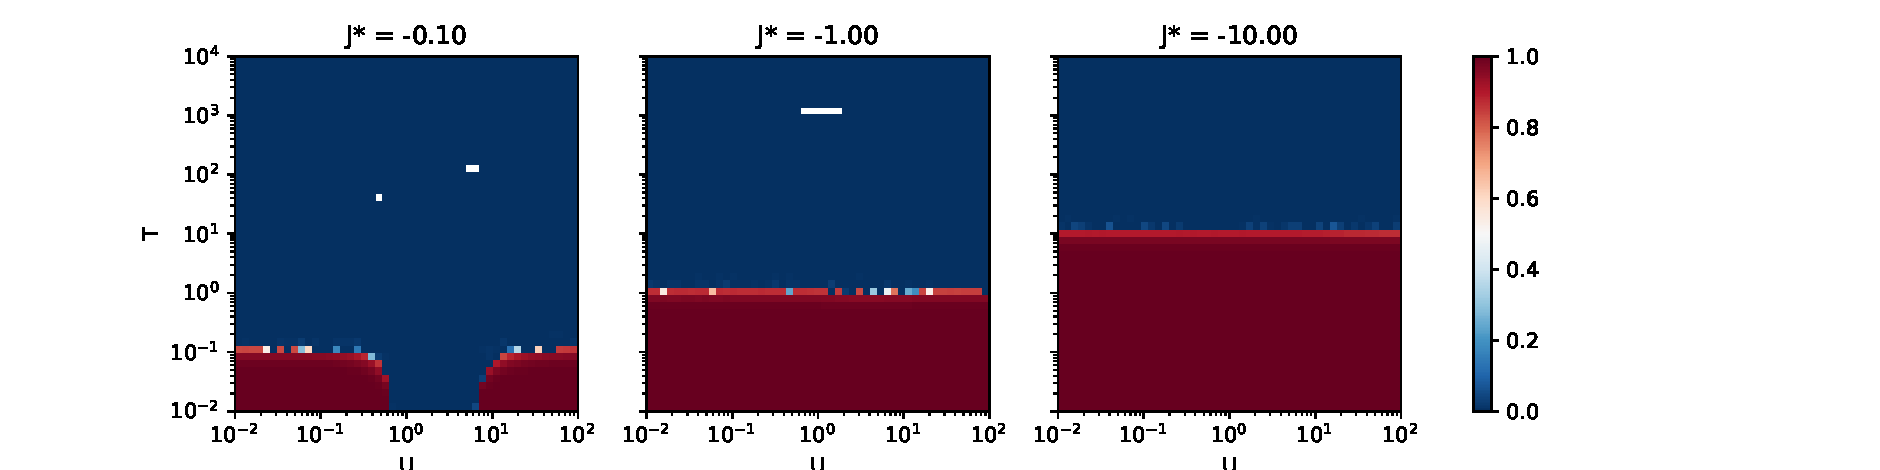
\includegraphics[width=\textwidth]{phase_diagram_4_log}
  \caption{A phase diagram of the full model with system size 128, $10^4$ MCMC steps and $alpha = 1.5$ The order parameter tracks the formation of the CDW phase. Strangely there seems to be a region around $U \approx 1$ for which the phase transition is suppressed. I'm not sure if this is a simulation artefact or not.}
  \label{fig:phase_diagram_4_log}
\end{figure}

\begin{figure}
  \centering
    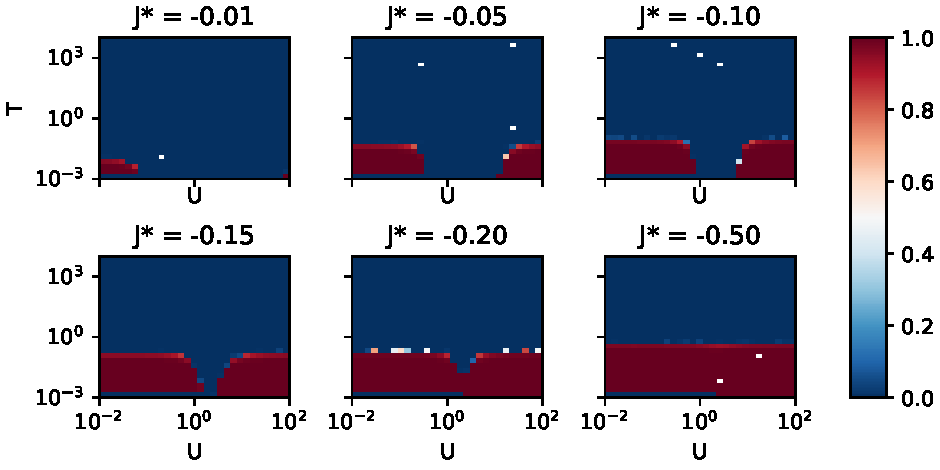
\includegraphics[width=1.2\textwidth]{phase_diagram_5_log}
  \caption{A phase diagram of the full model with system size 128, $10^4$ MCMC steps and $alpha = 1.5$ The order parameter tracks the formation of the CDW phase. This figure differs from Fig \ref{fig:states} in that the results are thermal averages obtained through MCMC.}
  \label{fig:phase_diagram_5_log}
\end{figure}

\section{Todo}
Articles from Johannes:

Are 1D phase transition driven by domain walls: https://www.sciencedirect.com/science/article/pii/S0167278906000418?via%3Dihub

Algorithm to construct potentials that show a mobility edge
Localization and the Mobility Edge in One-Dimensional Potentials with Correlated Disorder
https://journals.aps.org/prl/abstract/10.1103/PhysRevLett.82.4062

Review of localisation
http://www.phy.bme.hu/~zarand/LokalizacioWeb/Kramer.pdf

\subsection{Jan 18th Meeting with Jo}
\begin{itemize}
    \item Mean field theory for the ising model, repeat with coupling to the FK model
    \item Write up nematic order 
    \item look at A(d) and A(k) as defined by antipov
\end{itemize}

\subsection{Jan 23rd Meeting with Simon}
\begin{itemize}
    \item Gap at the fermi energy not enough to detect conductivity, need to look at the current-current response and kubo formula.
    \item Anderson insulator: finite DOS at fermi energy but no conducting (due to localisation?)
    \item Mott insulator like state in the 2D FK model is probably called that because in reference to a mott plateau in the density vs chemical potential curve. Simon pointed out that this is interesting because the insulating properties come entirely from the interactions rather than any reference to the bands.
\end{itemize}

\subsection{Jan 24th Meeting with Simon}
\begin{itemize}
    \item Asked about how particle hole symmetry, chirality and time reversal symmetry affect the band structure. 
\end{itemize}

\subsection{Feb 5th Meeting with Jo}
\begin{itemize}
    \item Particle hole <-> symmetric eigenenergies: Prove that particle hole is $PHP^\dagger = H$ then immediatly act with P on a wavefunction to get its partner with energy E
    \item FK Haldane model: 'Temperature driven gapless topological insulator'
    \item Compare particle hole to Kramers degeneracy
    \item For mean field calculations: 'competing orderings in an extended FK model' Brydon which has some stuff on MF
    \item Xiao-Gang Wan Quantum Field theory of many body systems has a good chapter on MF for the hubbard model called 'symmetry breaking in the spin density wave state'
 \end{itemize}
 
 https://github.com/Wookai/paper-tips-and-tricks


Document textwidth in inches: \printinunitsof{in}\prntlen{\textwidth}

\bibliographystyle{unsrt}
\bibliography{references}
\end{document}
